\documentclass{article}

\usepackage[utf8]{inputenc}
\usepackage[portuguese]{babel}
\usepackage{blindtext}
\usepackage{graphicx}
\usepackage{amsmath}
\usepackage{float}
\usepackage{caption}
\usepackage[compact]{titlesec}
\usepackage{multicol}
\usepackage[a4paper, total={7.5in, 10in}]{geometry}
\usepackage[font=scriptsize,labelfont=bf]{caption}
\usepackage{listings}
\usepackage{color}
 
\definecolor{codegreen}{rgb}{0,0.6,0}
\definecolor{codegray}{rgb}{0.5,0.5,0.5}
\definecolor{codepurple}{rgb}{0.58,0,0.82}
\definecolor{backcolour}{rgb}{0.95,0.95,0.92}
 
\lstdefinestyle{mystyle}{
    backgroundcolor=\color{backcolour},   
    commentstyle=\color{codegreen},
    keywordstyle=\color{magenta},
    numberstyle=\tiny\color{codegray},
    stringstyle=\color{codepurple},
    basicstyle=\footnotesize,
    breakatwhitespace=false,         
    breaklines=true,                 
    captionpos=b,                    
    keepspaces=true,                 
    numbers=left,                    
    numbersep=5pt,                  
    showspaces=false,                
    showstringspaces=false,
    showtabs=false,                  
    tabsize=2
}
 
\lstset{style=mystyle}

\setlength{\columnsep}{1cm}
\setlength{\parindent}{0em}
\titlespacing{\section}{1pt}{*-0.6}{*-1}
\begin{document}

\textbf{Relatório de Entrega de Trabalho} \newline
\textbf{Disciplina de Programação Paralela (PP)}\textbf{ - Prof. César De Rose} \newline
\textbf{Alunos:} Rafael Rios e Rodrigo Silveira \newline
\textbf{Exercício:} TPP2: MPI Divisão e Conquista (D\&C) \newline

\begin{multicols*}{2}

\section{Implementação}
O objetivo deste trabalho foi implementar um algoritmo de divisão e conquista para compreender aplicações paralelas, usando a biblioteca MPI, o problema proposto consiste em ordenar um vetor de 1000000 elementos, originalmente em ordem decrescente, para ordem crescente, utilizando o algoritmo bubblesort e quicksort. No inicio, o processo 0 cria o vetor enquanto os outros aguardam o recebimento do mesmo junto com a mensagem do tamanho do vetor recebido (MPI\_Get\_count). O processamento do que é feito com o vetor é realizado de modo igual por todos os processos no código, caso o tamanho do vetor recebido seja menor ou igual ao delta pré estabelecido, o vetor é ordenado, caso contrário, o vetor é separado e enviado para os filhos, que são escolhidos pelas fórmulas 2*(rank do processo)+1 e 2*(rank do processo)+2, garantindo a sequência na ordem dos processos. Outra implementação foi o controle para tamanhos de vetor não divisíveis por dois (Ex: 15625), quando isso ocorre, o filho da esquerda recebe a metade do vetor truncada (Ex: 7812) e o da direita a metade do vetor arredondada por excesso (Ex: 7813), esse controle é feito comparando o tamanho do vetor que os filhos receberão (float), com esse tamanho +0.5 truncado (int), caso for igual, ele é divisível por dois, caso contrário deve ser dividido como foi explicado. O mesmo código foi usado para a execução do algoritmo ordenado localmente pelos pais, antes de demonstrar o seu funcionamento, deve-se explicar duas variáveis: "tam\_local" é o tamanho que será executado localmente pelo pai e "tam\_divide" que é o tamanho a ser dividido igualmente pelos filhos, o controle é feito através de um valor definido (LOCAL), se for local, "tam\_local" recebe delta e "tam\_divide" recebe o tamanho do vetor subtraído pelo delta, se não for local, "tam\_local" recebe zero e "tam\_divide" recebe todo o tamanho do vetor a ser dividido. Após o envio do vetor para os filhos, se for o algoritmo com execução local, ele ordena a sua parte do vetor, depois, o pai recebe o vetor ordenado dos filhos (levando em conta se o tamanho enviado era divisível por dois) e organiza-o de modo a ficar ordenado, mostrando o tempo de execução no final, pelo processo 0.
\section{Dificuldades encontradas}
Elaboração de um método para garantir a ordem certa de envio dos vetores para os filhos, escolhendo quais processos receberiam o vetor; Resolução do problema para quando o tamanho do vetor não seria divisível por dois.
\section{Testes}
 O código foi executado para três casos com o intuito de mostrar as diferenças nos tempos de ordenamento. No primeiro teste o pai divide o vetor igualmente para os filhos até ser recebido o vetor com um tamanho menor ou igual a um delta pré estabelecido conforme o número de processos (caso A), sendo executado até 31 nodos (HT), em um segundo momento, o algoritmo foi testado para um número de processos maiores que o HT (caso C) e por último, realizou-se alterações no código para os pais ordenarem uma parte do vetor e dividir o resto para os filhos (caso B), com a finalidade de melhorar ainda mais o tempo de execução. Foram realizados testes com alocação de 2 nodos na grad, executando o algoritmo de divisão e conquista para 7, 15, 31, 63, 127 e 255 processos. O valor de delta para o caso B foi escolhido dividindo o tamanho do vetor pelo número de processos, de modo a balancear a ordenação dos vetores, já que cada processo fará a sua ordenação, para outros valores de delta usando uma porcentagem fixa, obtivemos resultados piores, visto que a ordenação ficava muito desbalanceada entre os processos. O delta para o caso A e C é dividido pela metade conforme aumenta-se o número de processos.
\section{Análise de desempenho}
Para o algoritmo quicksort, não houve uma mudança significativa nos tempos medidos, já que o algoritmo apresenta uma complexidade muito baixa. Entretanto, para o algoritmo bubblesort, notou-se que conforme aumentava-se o número de processos, o tempo de execução praticamente diminuía pela metade para todos os casos, mesmo passando do ponto de HT (pós 31 processos). O caso B com ordenação local obteve o melhor tempo de execução, visto que ao diminuir o tamanho do vetor a ser ordenado houve um menor gasto no bubblesort, agilizando o processo. Curiosamente, houve uma grande melhora no tempo de execução após o HT, mesmo havendo um número de processos maior do que o número de núcleos disponíveis. O speed-up melhorou com o aumento do número de processos para todos os casos, como mostra a Figura 1, e a eficiência estabilizou por volta de 4.0 após 15 processos para os casos A e C e em 13.0 para o caso B, também após 15 processos, com o tempo de execução diminuindo.
\begin{figure}[H]
            \centering
            \vspace{-1.1em}
            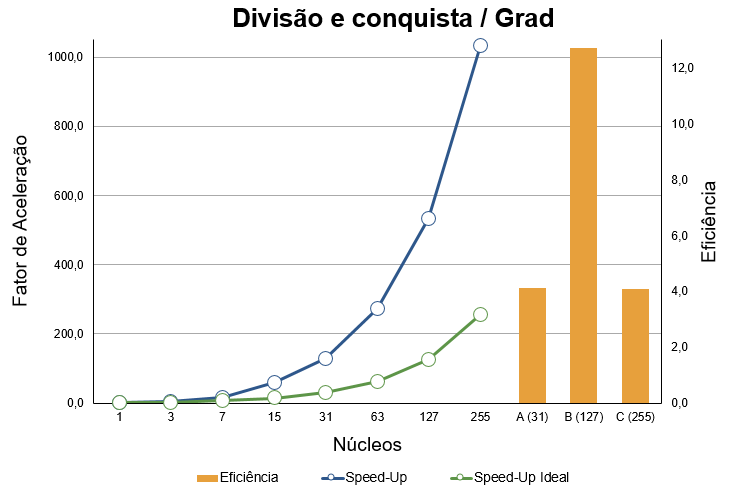
\includegraphics[width=9cm, height=4cm]{grafico.png}
            \vspace{-1.9em}
            \caption{Gráfico de Speed-up (A e C) e eficiência dos 3 casos}
            \vspace{-1.2em}
\end{figure}
\section{Observações Finais}
Apesar de o código ser extremamente compacto e simples, ele se mostrou muito eficiente, melhorando muito o tempo de execução do problema e apresentando um desempenho melhor que o mestre/escravo, já que não possui o gargalo de comunicação com o mestre. Notou-se a melhora no desempenho ao realizar a ordenação localmente, de modo a não deixar os processos pais ociosos e diminuindo o tamanho do vetor final a ser ordenado.

\end{multicols*}

\newpage

\lstinputlisting[language=C++]{tpp2.c}

\end{document}
